% Created by tikzDevice version 0.8.1 on 2015-06-10 21:23:14
% !TEX encoding = UTF-8 Unicode
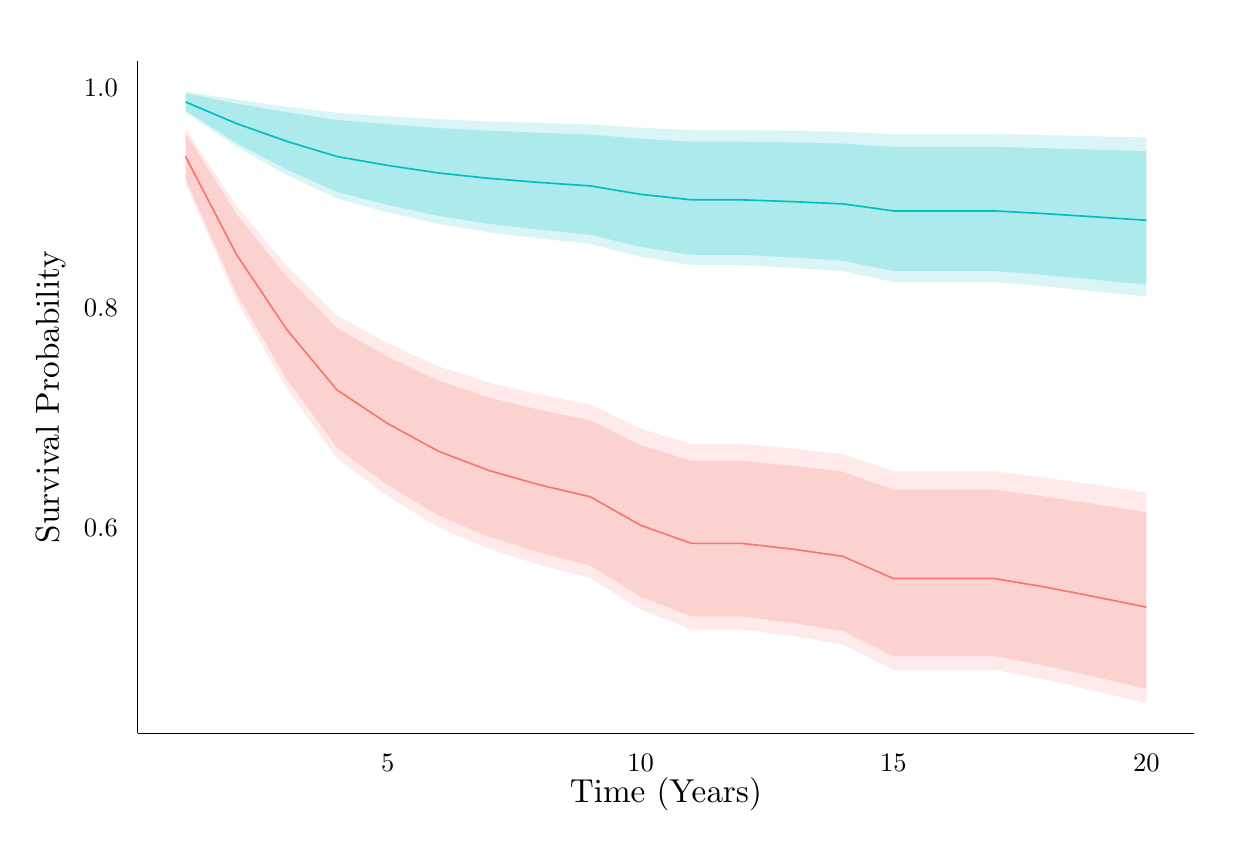
\begin{tikzpicture}[x=1pt,y=1pt]
\definecolor{fillColor}{RGB}{255,255,255}
\path[use as bounding box,fill=fillColor,fill opacity=0.00] (0,0) rectangle (433.62,289.08);
\begin{scope}
\path[clip] (  0.00,  0.00) rectangle (433.62,289.08);
\definecolor{drawColor}{RGB}{255,255,255}
\definecolor{fillColor}{RGB}{255,255,255}

\path[draw=drawColor,line width= 0.6pt,line join=round,line cap=round,fill=fillColor] (  0.00,  0.00) rectangle (433.62,289.08);
\end{scope}
\begin{scope}
\path[clip] ( 39.69, 34.03) rectangle (421.57,277.03);
\definecolor{fillColor}{RGB}{255,255,255}

\path[fill=fillColor] ( 39.69, 34.03) rectangle (421.58,277.03);
\definecolor{drawColor}{RGB}{248,118,109}

\path[draw=drawColor,line width= 0.6pt,line join=round] ( 57.05,242.57) --
	( 75.32,207.33) --
	( 93.59,180.03) --
	(111.86,158.08) --
	(130.13,146.00) --
	(148.41,136.03) --
	(166.68,129.05) --
	(184.95,123.88) --
	(203.22,119.59) --
	(221.49,109.27) --
	(239.77,102.74) --
	(258.04,102.74) --
	(276.31,100.65) --
	(294.58, 98.04) --
	(312.86, 90.01) --
	(331.13, 90.01) --
	(349.40, 90.01) --
	(367.67, 86.95) --
	(385.94, 83.39) --
	(404.22, 79.69);
\definecolor{drawColor}{RGB}{0,191,196}

\path[draw=drawColor,line width= 0.6pt,line join=round] ( 57.05,262.24) --
	( 75.32,254.49) --
	( 93.59,248.02) --
	(111.86,242.49) --
	(130.13,239.30) --
	(148.41,236.58) --
	(166.68,234.63) --
	(184.95,233.15) --
	(203.22,231.91) --
	(221.49,228.86) --
	(239.77,226.87) --
	(258.04,226.87) --
	(276.31,226.22) --
	(294.58,225.41) --
	(312.86,222.86) --
	(331.13,222.86) --
	(349.40,222.86) --
	(367.67,221.87) --
	(385.94,220.70) --
	(404.22,219.47);
\definecolor{fillColor}{RGB}{248,118,109}

\path[fill=fillColor,fill opacity=0.15] ( 57.05,252.56) --
	( 75.32,224.83) --
	( 93.59,202.93) --
	(111.86,185.04) --
	(130.13,175.05) --
	(148.41,166.70) --
	(166.68,160.79) --
	(184.95,156.48) --
	(203.22,152.88) --
	(221.49,144.20) --
	(239.77,138.68) --
	(258.04,138.68) --
	(276.31,137.00) --
	(294.58,134.98) --
	(312.86,128.79) --
	(331.13,128.79) --
	(349.40,128.79) --
	(367.67,126.45) --
	(385.94,123.85) --
	(404.22,121.13) --
	(404.22, 45.08) --
	(385.94, 49.38) --
	(367.67, 53.53) --
	(349.40, 57.05) --
	(331.13, 57.05) --
	(312.86, 57.05) --
	(294.58, 66.24) --
	(276.31, 69.26) --
	(258.04, 71.60) --
	(239.77, 71.60) --
	(221.49, 78.79) --
	(203.22, 90.22) --
	(184.95, 94.98) --
	(166.68,100.77) --
	(148.41,108.53) --
	(130.13,119.71) --
	(111.86,133.42) --
	( 93.59,158.70) --
	( 75.32,190.70) --
	( 57.05,232.85) --
	cycle;
\definecolor{fillColor}{RGB}{0,191,196}

\path[fill=fillColor,fill opacity=0.15] ( 57.05,265.99) --
	( 75.32,263.05) --
	( 93.59,260.53) --
	(111.86,258.33) --
	(130.13,257.06) --
	(148.41,255.99) --
	(166.68,255.22) --
	(184.95,254.62) --
	(203.22,254.12) --
	(221.49,252.88) --
	(239.77,252.08) --
	(258.04,252.08) --
	(276.31,251.82) --
	(294.58,251.51) --
	(312.86,250.58) --
	(331.13,250.58) --
	(349.40,250.58) --
	(367.67,250.24) --
	(385.94,249.83) --
	(404.22,249.40) --
	(404.22,191.90) --
	(385.94,193.81) --
	(367.67,195.61) --
	(349.40,197.16) --
	(331.13,197.16) --
	(312.86,197.16) --
	(294.58,201.09) --
	(276.31,202.34) --
	(258.04,203.32) --
	(239.77,203.32) --
	(221.49,206.34) --
	(203.22,210.99) --
	(184.95,212.88) --
	(166.68,215.14) --
	(148.41,218.15) --
	(130.13,222.35) --
	(111.86,227.29) --
	( 93.59,235.91) --
	( 75.32,246.11) --
	( 57.05,258.52) --
	cycle;
\definecolor{fillColor}{RGB}{248,118,109}

\path[fill=fillColor,fill opacity=0.20] ( 57.05,250.94) --
	( 75.32,221.95) --
	( 93.59,199.13) --
	(111.86,180.54) --
	(130.13,170.18) --
	(148.41,161.54) --
	(166.68,155.44) --
	(184.95,150.97) --
	(203.22,147.25) --
	(221.49,138.26) --
	(239.77,132.55) --
	(258.04,132.55) --
	(276.31,130.79) --
	(294.58,128.66) --
	(312.86,122.12) --
	(331.13,122.12) --
	(349.40,122.12) --
	(367.67,119.65) --
	(385.94,116.86) --
	(404.22,113.95) --
	(404.22, 50.23) --
	(385.94, 54.46) --
	(367.67, 58.54) --
	(349.40, 61.99) --
	(331.13, 61.99) --
	(312.86, 61.99) --
	(294.58, 71.04) --
	(276.31, 74.00) --
	(258.04, 76.31) --
	(239.77, 76.31) --
	(221.49, 83.41) --
	(203.22, 94.70) --
	(184.95, 99.40) --
	(166.68,105.10) --
	(148.41,112.75) --
	(130.13,123.76) --
	(111.86,137.24) --
	( 93.59,162.03) --
	( 75.32,193.31) --
	( 57.05,234.40) --
	cycle;
\definecolor{fillColor}{RGB}{0,191,196}

\path[fill=fillColor,fill opacity=0.20] ( 57.05,265.38) --
	( 75.32,261.66) --
	( 93.59,258.49) --
	(111.86,255.74) --
	(130.13,254.15) --
	(148.41,252.80) --
	(166.68,251.83) --
	(184.95,251.09) --
	(203.22,250.46) --
	(221.49,248.92) --
	(239.77,247.91) --
	(258.04,247.91) --
	(276.31,247.59) --
	(294.58,247.19) --
	(312.86,245.98) --
	(331.13,245.98) --
	(349.40,245.98) --
	(367.67,245.53) --
	(385.94,244.99) --
	(404.22,244.42) --
	(404.22,196.18) --
	(385.94,197.99) --
	(367.67,199.70) --
	(349.40,201.16) --
	(331.13,201.16) --
	(312.86,201.16) --
	(294.58,204.88) --
	(276.31,206.07) --
	(258.04,207.00) --
	(239.77,207.00) --
	(221.49,209.86) --
	(203.22,214.27) --
	(184.95,216.06) --
	(166.68,218.20) --
	(148.41,221.05) --
	(130.13,225.02) --
	(111.86,229.69) --
	( 93.59,237.83) --
	( 75.32,247.44) --
	( 57.05,259.11) --
	cycle;
\end{scope}
\begin{scope}
\path[clip] (  0.00,  0.00) rectangle (433.62,289.08);
\definecolor{drawColor}{RGB}{0,0,0}

\path[draw=drawColor,line width= 0.6pt,line join=round] ( 39.69, 34.03) --
	( 39.69,277.03);
\end{scope}
\begin{scope}
\path[clip] (  0.00,  0.00) rectangle (433.62,289.08);
\definecolor{drawColor}{RGB}{0,0,0}

\node[text=drawColor,anchor=base east,inner sep=0pt, outer sep=0pt, scale=  0.96] at ( 32.57,105.05) {0.6};

\node[text=drawColor,anchor=base east,inner sep=0pt, outer sep=0pt, scale=  0.96] at ( 32.57,184.54) {0.8};

\node[text=drawColor,anchor=base east,inner sep=0pt, outer sep=0pt, scale=  0.96] at ( 32.57,264.03) {1.0};
\end{scope}
\begin{scope}
\path[clip] (  0.00,  0.00) rectangle (433.62,289.08);
\definecolor{drawColor}{RGB}{0,0,0}

\path[draw=drawColor,line width= 0.6pt,line join=round] ( 39.69, 34.03) --
	(421.57, 34.03);
\end{scope}
\begin{scope}
\path[clip] (  0.00,  0.00) rectangle (433.62,289.08);
\definecolor{drawColor}{RGB}{0,0,0}

\node[text=drawColor,anchor=base,inner sep=0pt, outer sep=0pt, scale=  0.96] at (130.13, 20.31) {5};

\node[text=drawColor,anchor=base,inner sep=0pt, outer sep=0pt, scale=  0.96] at (221.49, 20.31) {10};

\node[text=drawColor,anchor=base,inner sep=0pt, outer sep=0pt, scale=  0.96] at (312.86, 20.31) {15};

\node[text=drawColor,anchor=base,inner sep=0pt, outer sep=0pt, scale=  0.96] at (404.22, 20.31) {20};
\end{scope}
\begin{scope}
\path[clip] (  0.00,  0.00) rectangle (433.62,289.08);
\definecolor{drawColor}{RGB}{0,0,0}

\node[text=drawColor,anchor=base,inner sep=0pt, outer sep=0pt, scale=  1.20] at (230.63,  9.03) {Time (Years)};
\end{scope}
\begin{scope}
\path[clip] (  0.00,  0.00) rectangle (433.62,289.08);
\definecolor{drawColor}{RGB}{0,0,0}

\node[text=drawColor,rotate= 90.00,anchor=base,inner sep=0pt, outer sep=0pt, scale=  1.20] at ( 11.28,155.53) {Survival Probability};
\end{scope}
\end{tikzpicture}
